\documentclass[10pt,a4paper, twocolumn]{report}
\usepackage[T1]{fontenc} 
\usepackage[utf8]{inputenc} 
\usepackage[spanish]{babel}
\usepackage{amsmath}
\usepackage{amsfonts}
\usepackage{amssymb}
\usepackage{graphicx}
\author{Antonio Molina Garca-Retamero}
\title{Results report}
\makeindex
\begin{document}
\maketitle
\pagebreak
\tableofcontents
\pagebreak
\section{Results for classification in clustered data set}
In this section we'll perform a test battery in order to determine how well works the neural network by classifying data in a clustered data set.
For each test, we test the accuracy of the prediction for a determine data set clustered in k centroids and the time elapsed in training phase. We will increase the number of neurons in first layer for each test
\subsection{For k clusters and n samples}
\begin{figure}[!h]{}
    \centering
    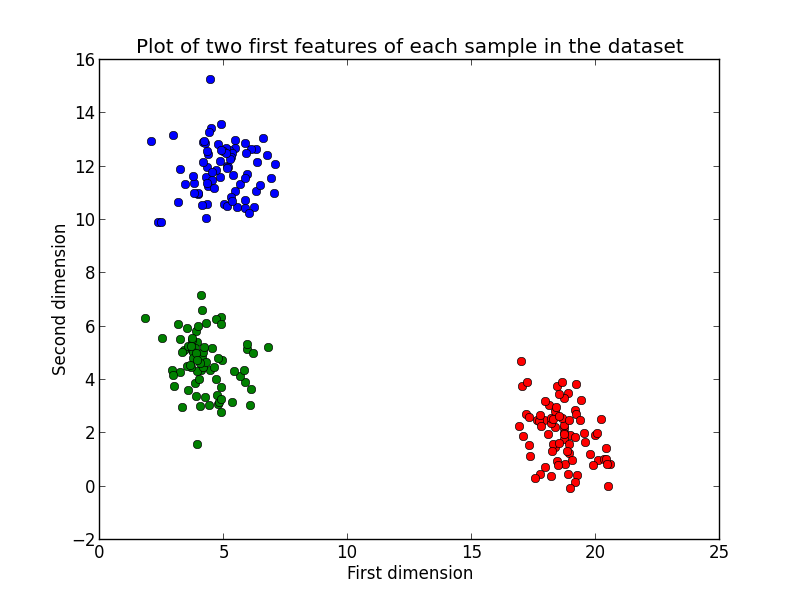
\includegraphics[width=0.4\textwidth]{plots/3c100s.png}
    \label{fig:clusteredData1}
\end{figure}
\begin{tabular}{|l | c | r|}
\hline
\hline
Centroids & Performance & Training time \\
\hline
col 1 & col 2 & col 3\\
\hline
\end{tabular}
